%%%%%%%%%%%%%%%%% Modelo de Ashkin-Teller %%%%%%%%%%%%%%%%%%%%%%%%


\subsection{Definición del modelo.}
\label{sec:AT_model}

El modelo de Ashkin-Teller fue introducido en el año 1943 \cite{ashkin_teller_43} como una generalización del modelo de Ising.
 Consiste en una red cuadrada bidimensional donde 4 tipos de átomos ($A$, $B$, $C$ y $D$) interactúan a primeros vecinos, la energía de
 interacción depende de los átomos involucrados: $\epsilon_{0}$ para $AA$, $BB$, $CC$, $DD$; $\epsilon_{1}$ para $AB$, $CD$;
 $\epsilon_{2}$ para $AC$, $BD$; y $\epsilon_{3}$ para $AD$, $BC$.\\
Este modelo no ha sido resuelto analíticamente, sin embargo algunas de sus propiedades críticas son conocidas exactamente por medio de relaciones con otros modelos, principalmente
 el mapeo al modelo de Gas de Coulomb \cite{cardy_book}.\\
Fan \cite{AT_fan1972b} ha demostrado que asociando dos spines $\sigma_{ij}$, $\tau_{ij}$ a cada sitio $ij$ en la red y asignando un estado de este par de spines
 a cada tipo de átomo ($A\rightarrow (+,+)$, $B\rightarrow (+,-)$, $C\rightarrow (-,+)$, y $D\rightarrow (-,-)$), el modelo
 puede representarse como dos modelos de Ising ($\sigma$ y $\tau$) acoplados con una interacción entre cuatro spines ($\sigma_{ij}\sigma_{km}\tau_{ij}\tau_{km}$):
\\
\begin{equation}
	\label{eq:ham_AT}
	H_{AT}=-\sum_{<ij,km>}(J\sigma_{ij}\sigma_{km}+J'\tau_{ij}\tau_{km})-J_{4}\sum_{<ij,km>}\sigma_{ij}\sigma_{km}\tau_{ij}\tau_{km}
\end{equation}
donde los pares de índices $i,j$ y $k,m$ numeran los sitios en una red bidimensional y el símbolo $<ij,km>$ indica que las sumatorias son a primeros
 vecinos en la red. $J$ y $J'$ son las instensidades de las interacciones entre spines del mismo tipo, $\sigma$-$\sigma$ y $\tau$-$\tau$, respectivamente y
  $J_{4}$ es la intensidad de la interacción de cuatro spines.
 Estas constantes de acoplamiento resultan combinaciones lineales sencillas de las originales ($\epsilon_{0}$,$\epsilon_{1}$,$\epsilon_{2}$ y $\epsilon_{3}$).\\
Considerando el caso $J_{4}=0$ puede verse que el sistema se separa en dos modelos de Ising con constantes de acoplamiento diferentes, y por lo
 tanto con dos temperaturas críticas. Esto condujo a Wegner \cite{AT_wegner} a relacionar el modelo AT con el modelo 8V a través de una transformación
 de dualidad realizada solo sobre los spines $\sigma$, dando los primeros indicios sobre la riqueza de su comportamiento crítico.\\
Se ha determinado que para $J \neq J'$ el modelo AT pertenece a la clase de universalidad del modelo de Ising bidimensional, sin embargo en el caso
 isotrópico, es decir cuando $J=J'$, exhibe una dependencia de los exponentes críticos con el acoplamiento $J_{4}$, lo cual significa que presenta características
 no universales. Esta situación fue estudiada fuertemente por Kadanoff \cite{AT8V_kadanoff_1977} (utilizando álgebra de operadores) y Brown (mediante la teoría de escala
 y el grupo de renormalización). Las siguientes expresiones fueron halladas para los exponentes críticos:
\\
\begin{equation}
	\label{eq:AT_crit_exps}
	\alpha =\frac{(2-2y)}{(3-2y)},\beta_{m}=\frac{(2-y)}{(24-16y)},\beta_{e}=\frac{1}{(12-8y)}
\end{equation}
\\

 donde $\alpha$ es el exponente del calor específico, $\beta_{m}$ de la magnetización $\mean{\sigma}$ y $\beta_{e}$ de la magnetización asociada al
 producto de los spines $\sigma$ y $\tau$, $\mean{\sigma\tau}$. La dependencia de los exponentes cr\'iticos con el acoplamiento $J_{4}$ est\'a contenida,
 en estas ecuaciones, en el par\'ametro $y=2\mu /\pi$, con $\cos(\mu)=\frac{1}{2}(e^{4K_{4}}-1)$ y $K_{4}=J_{4}/kT$.\\

\begin{figure}[h!]
\begin{center}
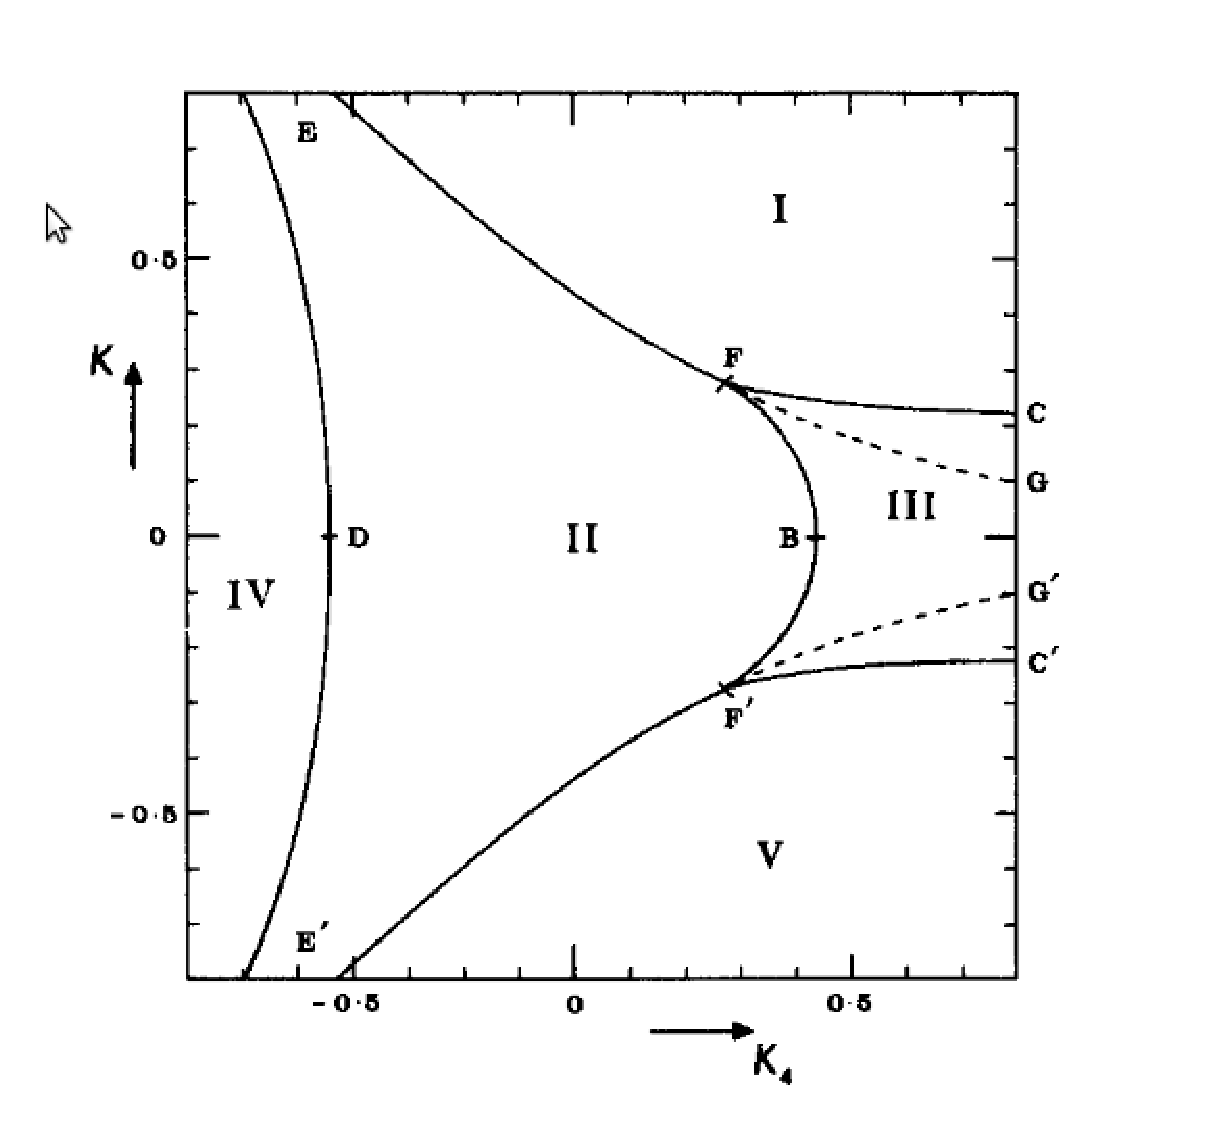
\includegraphics[scale=0.65]{graf/phases/AT_ph_diag_Baxter.eps}
\end{center}
\caption{Diagrama de fases del modelo Ashkin-Teller. El sistema se encuentra en diferentes estados de orden en cada una de las regiones I, II, III, IV y V.
 Se indican con letras (B, C, C$'$, D, E, E$'$, F, F$'$, G, G$'$) algunos puntos en los que $K_{4}$ y $K$ son conocidos exactamente.}
\label{fig:AT_ph_diag_Baxter}
\end{figure}

El diagrama de fases del modelo AT representado en la figura \ref{fig:AT_ph_diag_Baxter} en t\'erminos de $K=J/kT$ y $K_{4}=J_{4}/kT$,
 fue obtenido, utilizando resultados que surgieron de varios métodos (simulaciones MC, teoría de campo medio y grupo de renormalización),
 en 1980 por Ditzian et. al. \cite{AT_3D_phdiag}. En él se evidencian cinco regiones caracterizadas por diferentes estados de orden.\\
Además de los parámetros de orden usuales para un sistema magnético dados en la sección \ref{sec:teoria}, es útil definir unos que midan el grado de orden entre
ambos tipos de spines, gobernado por el acoplamiento $K_{4}$, para ello consideraremos el momento magnético dado por el producto $\sigma\tau$:

\begin{center} 
\begin{eqnarray}
	\label{eq:op_Mst}
	\mean{\sigma\tau}&=&\frac{1}{L^{2}}\sum_{ij}\sigma_{ij}\tau_{ij} \\
	\label{eq:op_stagMst}
	\mean{\sigma\tau}_{AF}&=&\frac{1}{L^{2}}\sum_{ij}(-1)^{(i+j)}\sigma_{ij}\tau_{ij}
\end{eqnarray}
\end{center}
 donde $ij$ representa los \'indices de un sitio en la red bidimensiional y las sumatorias se extienden sobre toda la red.
El parámetro de orden $\mean{\sigma \tau}$ es una medida de la proporci\'on de pares de spines $\sigma-\tau$ en los que $\sigma$ y $\tau$
 se encuentran alineados en el mismo sitio de red, toma su valor máximo solo cuando los spines en ambos planos se encuentran en el mismo estado de orden;
 $\mean{\sigma\tau}_{AF}$ mide el orden alternado de los pares $\sigma-\tau$,
 este par\'ametro puede ser no nulo incluso cuando $\mean{\sigma}$ y $\mean{\tau}$ son ambos nulos.\\

En la regi\'on I del diagrama de fases de la fig. \ref{fig:AT_ph_diag_Baxter} ambos acoplamientos, $K$ y $K_{4}$, son suficientemente fuertes, $\mean{\sigma}$ y $\mean{\tau}$ est\'an ordenandos de forma independiente
 ($\mean{\sigma}=\pm \mean{\tau}$) y $\mean{\sigma\tau}$ es no nulo, y por lo tanto,% esto ocurre cuando $K_{4}/K \gtrsim -1$ y
 el sistema presenta orden ferromagn\'etico total. En la regi\'on II, los acoplamientos son muy d\'ebiles y el sistema est\'a
 completamente desordenado ($\mean{\sigma}$, $\mean{\tau}$ y $\mean{\sigma\tau}$ son nulos).
La regi\'on III presenta orden parcial, $K_{4}$ supera a $K$ en toda la regi\'on, permitiendo que $\sigma\tau$ presente orden ferromagn\'etico mientras que $\tau$ y $\sigma$
 est\'an independientemente desordenados.
La regi\'on IV se da para valores grandes y negativos de $K_{4}$ los spines $\sigma$ y $\tau$ se encuentran desordenados, mientras que $\sigma\tau$ presenta orden de tipo anti-ferromagn\'etico.
La región V es similar a la I, pero $\sigma$ y $\tau$ están ordenados de manera anti-ferromagnética.\\

La curva E-F que delimita las regiones I y II en el diagrama de fases de la Fig. \ref{fig:AT_ph_diag_Baxter} resulta de particular interés, ya que
 sobre ella los exponentes críticos del modelo varian continuamente con el acoplamiento $K_{4}$. La expresión analítica que define dicha curva
 en términos de las constantes de acoplamiento del modelo AT \cite{AT_fan1972a,baxter_book} puede obtenerse a partir de un análisis de simetrías sobre el modelo 8V
 y está dada por:
\\ 
\begin{equation}
	\label{eq:lincrit}
	e^{(-2K_{4})}=\sinh{(2K)} , \; \; \; \; K_{4}<K,
\end{equation}
\\
 el punto E corresponde a $K_{4}/K =-1$, $K\rightarrow\infty$, donde $\mu=2\pi/3$, y el punto F a $K_{4}=K$, con $\mu=0$.\\
Si se analiza el caso $K_{4}=0$, se obtiene el punto crítico $K=K_{c}^{Ising}$ para el modelo de Ising, donde $K_{c}^{Ising}$ está dado por:
\\
\begin{equation}
	\label{eq:isingcrit}
	\sinh{(2K_{c}^{Ising})}=1, %\; \; \; \; K_{c}^{Ising}\eqsim 0.440686...
\end{equation}
\\
Respecto a las curvas que separan el resto de las fases en el diagrama de la fig. \ref{fig:AT_ph_diag_Baxter}, sólo la curva E$'$-F$'$,
 que se obtiene a partir de la línea E-F negando $K$, es conocida analíticamente, y sobre ella los exponentes críticos varian continuamente.
 Las prolongaciones F-G y F$'$-G$'$ (en líneas punteadas en la fig. \ref{fig:AT_ph_diag_Baxter}) no representan
 curvas críticas. Si bien las curvas F-B y F-C no son conocidas analíticamente, el punto B ha sido estimado como $K=0$, $K_{4}=K_{c}^{Ising}$ y el punto C es
 $K_{4}=\infty$, $K=\frac{1}{2}K_{c}^{Ising}$. De la misma forma, la curva E-D-E$'$ no es conocida anal\'iticamente, pero el punto D corresponde a $K=0$, $K_{4}=-K_{c}^{Ising}$.
 Los exponentes críticos sobre estas tres últimas curvas tienen valores fijos, y se espera que estos sean los del modelo de Ising bidimensional.\\
